\documentclass[11pt,a4paper]{article}
\usepackage[ngerman]{babel}
\usepackage[TS1,T1]{fontenc}
\usepackage[utf8x]{inputenc}
\selectlanguage{ngerman}
\usepackage{theorem}
\usepackage[scaled=0.9]{helvet}
\usepackage{amsmath}
\usepackage{amssymb}
\usepackage{hyperref}
\usepackage{stmaryrd}
\usepackage{pgf,tikz}
\usepackage{relsize}
\usepackage{enumitem}
\usepackage{graphicx}
\usepackage{algpseudocode,amsmath,xifthen}

\newcounter{numb}
\theoremstyle{break}
\theorembodyfont{\upshape}
   	\newtheorem{exercise}{Exercise}[numb]
\setlength{\oddsidemargin}{0cm}
\setlength{\textwidth}{16cm}
\setlength{\textheight}{23cm}
\setlength{\topmargin}{-2cm}

\usetikzlibrary{shapes,arrows,automata,positioning,decorations.fractals}
\renewcommand\familydefault{\sfdefault}

\newcommand{\header}[2]{
\begin{minipage}[b]{\textwidth}
		\parbox[t]{5cm}{%
			
\includegraphics[width=4cm]{unilogo}
			\hfill
		}
		\parbox[b]{11cm}{%
			%\scshape%
			Heinrich-Heine-University D\"usseldorf\\
			Computer Science Department\\
			Software Engineering and Programming Languages\\
			%Professor Dr.\ M.\ Leuschel
		Philipp K\"orner
}
		
\end{minipage}
	\begin{center}
		\bf
		Functional Programming -- WT 2024 / 2025\\
        Reading Guide {\thenumb}: {#1}
	\end{center}

    \pagestyle{empty}
    \paragraph{Timeline:} This unit should be completed by {#2}.
}

\setcounter{numb}{5}


\begin{document}
	
	\begin{minipage}[b]{\textwidth}
		\parbox[t]{5cm}{%
			
\includegraphics[width=4cm]{unilogo}
			\hfill
		}
		\parbox[b]{11cm}{%
			%\scshape%
			Heinrich-Heine-University D\"usseldorf\\
			Computer Science Department\\
			Software Engineering and Programming Languages\\
			%Professor Dr.\ M.\ Leuschel
			Philipp K\"orner
		}
	\end{minipage}
\begin{center}
	\bf
	Functional Programming -- WT 2021 / 2022\\
    Reading Guide 5: Recursion, Destructuring \& More
\end{center}

\pagestyle{empty}

\paragraph{Timeline:} This unit should be completed by 15.11.2021.

\section{Material} 

\begin{itemize}
\item 05\_recursion.clj 
\item 04\_destructuring.clj
\item 07\_java\_interop.clj
\item 08\_namespaces.clj
\item 09\_evaluation\_order.clj
\end{itemize}

\paragraph{Note:} This unit groups several REPL sessions.
The focus lies on understanding explicit recursion and destructuring.
While the code volume is larger than usual,
the REPL sessions do not introduce complex concepts
and require less cognitive load.
In particular, we do not expect you to be able to write programs interacting heavily with Java
or to name all internal mappings of a namespace.
Nonetheless, you should be aware of the basic mechanisms
and might be required to work with them later on.

\section{Learning Outcomes}

After completing this unit you should be able to

\begin{itemize}
    \item write recursive programs yourself.
    \item read destructurings of data structures and specify the binding of symbols.
    \item be able to read Host interop forms.
    \item roughly sketch how namespaces work.
    \item know in which order symbols are evaluted.
\end{itemize}

\section{Highlights}

\begin{itemize}
    \item Destructuring
    \item Special Forms: \verb|loop|, \verb|recur|
    \item Functions: \verb|trampoline|
\end{itemize}



\section{Exercises}
\begin{exercise}[Hash Trie]

	In this exercise we consider a hash trie with a branching factor of 4,
	meaning every node has at most 4 children.
	Assume the following hash values for this exercise:

    \begin{center}
    \begin{tabular}{l@{}ll@{}l}
        hash(:a)    &= \colorbox{red!15}{00}\colorbox{blue!15}{10}\colorbox{orange!15}{00}\colorbox{green!15}{00} &hash(:e)    &= \colorbox{red!15}{10}\colorbox{blue!15}{01}\colorbox{orange!15}{11}\colorbox{green!15}{01}\\
        hash(:b)    &= \colorbox{red!15}{10}\colorbox{blue!15}{00}\colorbox{orange!15}{00}\colorbox{green!15}{10} &hash(:new)  &= \colorbox{red!15}{00}\colorbox{blue!15}{01}\colorbox{orange!15}{01}\colorbox{green!15}{10}\\
        hash(:c)    &= \colorbox{red!15}{01}\colorbox{blue!15}{11}\colorbox{orange!15}{10}\colorbox{green!15}{10} &hash(:ouch) &= \colorbox{red!15}{11}\colorbox{blue!15}{01}\colorbox{orange!15}{11}\colorbox{green!15}{01}\\
        hash(:d)    &= \colorbox{red!15}{11}\colorbox{blue!15}{00}\colorbox{orange!15}{01}\colorbox{green!15}{00} &\\
    \end{tabular}
    \end{center}

\begin{center}
    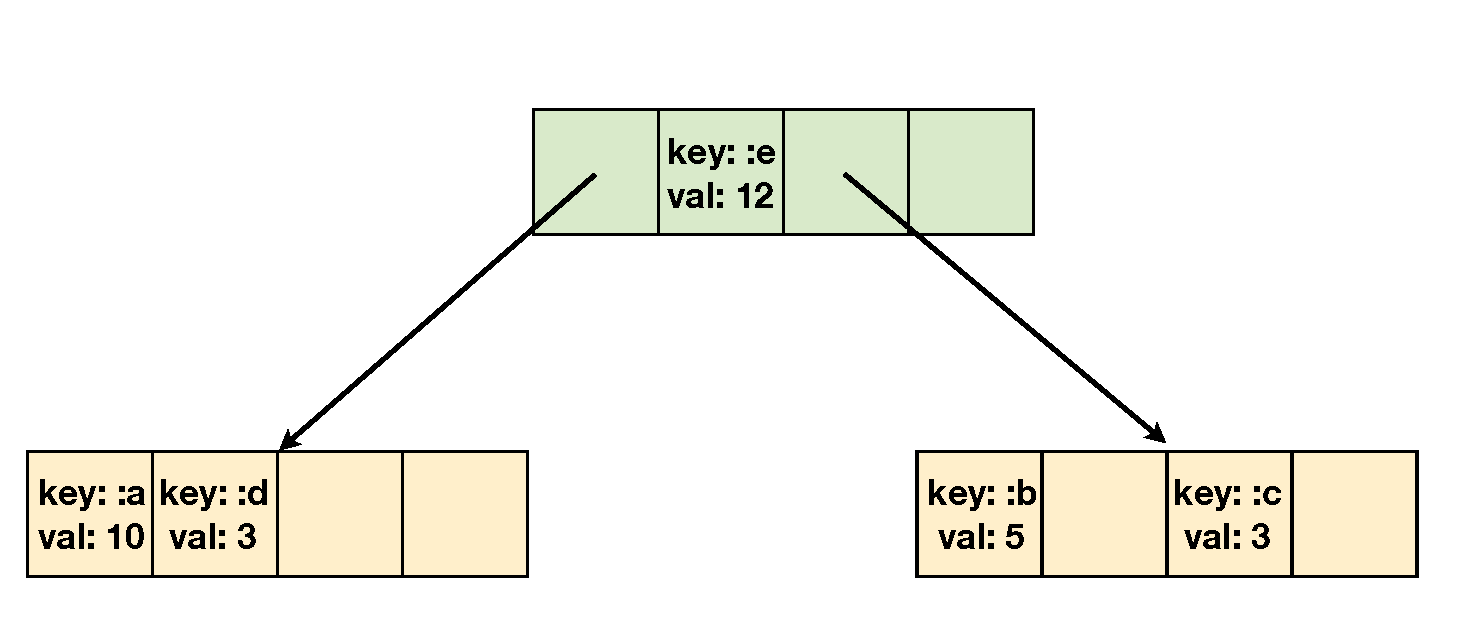
\includegraphics[scale=0.4]{hashtrie.pdf}
\end{center}

\begin{enumerate}[label=\alph*)]
\item
	Which map is stored in the pictured trie?
\item
	How many bits are needed for determining the position in an array?
\item
	Insert the value \texttt{:ez} under key \texttt{:new}.
	Which nodes can be referenced in the previous trie and which have to be copied?
\item
	Insert the value \texttt{:almost-a-collision} under key \texttt{:ouch}.
	Which nodes can be referenced in the previous trie and which have to be copied?
\end{enumerate}
\end{exercise}


\pagebreak

\begin{exercise}[Maxima]

\begin{enumerate}[label=\alph*)]
\item
  Define a function, that returns the maximum of its arguments.
\begin{verbatim}
(max-value 3 42 1336 12.5)
=> 1336
\end{verbatim}
\item
  Define a function that returns the first, longest sequence of its arguments. Nesting should not be considered.
\begin{verbatim}
(longest []  [:a :b 12] [[1 2 3 4 5 6]])
=> [:a :b 12]
\end{verbatim}
\item
  Define a function that determines the maximal length of its arguments. Nesting should not be considered.
\begin{verbatim}
(max-length []  [:a :b 12] [[1 2 3 4 5 6]])
=> 3
\end{verbatim}

\end{enumerate}
\end{exercise}



\begin{exercise}[Matrix]
In the following exercise, we consider a matrix as a vector of row vectors. For example:
\begin{verbatim}
(def identity-matrix [[1 0 0] [0 1 0] [0 0 1]])
(def matrix2 [[1 0 0 1] [0 1 0 1] [0 0 1 1]])
\end{verbatim}

\begin{enumerate}[label=\alph*)]
\item Write a function \verb|p!|, which outputs the matrix.
\begin{verbatim}
user=> (p! identity-matrix)
100
010
001
\end{verbatim}
  
\item Write a function \verb|trans|, which transposes the matrix, i.e. swaps the rows and columns:
\begin{verbatim}
user=> (= identity-matrix (trans identity-matrix))
true
user=> (p! (trans matrix2))
100
010
001
111
user=> (= matrix2 (trans matrix2))
false
user=> (= matrix2 (trans (trans matrix2)))
true 
\end{verbatim}
\end{enumerate}

\end{exercise}

\begin{exercise}[Black Box Testing (4clojure \#65)]
	Clojure has different collections, which differ (slightly) in their behaviour.
	Functions in \verb|clojure.core| typically transform them into sequences and work on them.
	It is nonetheless important to understand the differences in behaviour and performance 
	to choose an appropriate representation for given data.

    Write a function \verb|data-type|, which takes a collection as parameter and returns \verb|:map|, \verb|:set|, \verb|:list| or \verb|:vector|
    depending on which type of collection was passed.

	It is prohibited to use the \verb|list?| predicate.
	The point of this exercise is to play around with collections and understand their behaviour.
\end{exercise}

\section*{Questions}
If you have any questions, please contact Philipp K"orner (\texttt{p.koerner@hhu.de}).
\end{document}

